\documentclass[UTF8,fontset=fandol,11pt]{ctexart}
\usepackage[a4paper,margin=24mm,headheight=15pt]{geometry}
\usepackage{amsmath,amssymb,amsthm,mathtools,bm}
\usepackage{enumitem,booktabs,longtable,array,pdfpages,fancyhdr,xcolor}
\usepackage[colorlinks=true,linkcolor=blue!45!black,urlcolor=blue!45!black]{hyperref}
\allowdisplaybreaks[2]
\setlength{\parindent}{2em}
\setlength{\parskip}{3pt}
\setlength{\emergencystretch}{3em}
\setlist{nosep,topsep=3pt}
\pagestyle{fancy}\fancyhf{}\fancyhead[L]{\small 分析学讲义习题解答}\fancyhead[R]{\small 第38--57讲}\fancyfoot[C]{\thepage}
\newcommand{\R}{\mathbb R}\newcommand{\C}{\mathbb C}\newcommand{\N}{\mathbb N}\newcommand{\Z}{\mathbb Z}\newcommand{\Q}{\mathbb Q}\newcommand{\T}{\mathbb T}
\newcommand{\dd}{\,\mathrm d}\newcommand{\eps}{\varepsilon}\newcommand{\ind}{\mathbf1}
\newcommand{\norm}[1]{\left\lVert#1\right\rVert}\newcommand{\abs}[1]{\left|#1\right|}\newcommand{\ip}[2]{\left\langle#1,#2\right\rangle}
\DeclareMathOperator{\supp}{supp}\DeclareMathOperator{\rank}{rank}\DeclareMathOperator{\Span}{Span}\DeclareMathOperator{\diag}{diag}\DeclareMathOperator{\Res}{Res}\DeclareMathOperator{\Ext}{Ext}
\newcommand{\problem}[2]{\subsection*{#1}\addcontentsline{toc}{subsection}{#1}\noindent\textbf{题干。}#2\par\smallskip\noindent\textbf{解答。}}
\newcommand{\fix}[1]{\par\noindent\textcolor{red!55!black}{\textbf{原文核对与修正。}#1}\par}
\newcommand{\skipnote}[1]{\par\noindent\textbf{依约不解的计算题。}#1\par}
\newcommand{\sourceintro}[3]{\title{#1\\[4pt]\large 题干、解答与勘误}\author{于品《数学分析讲义》配套解答}\date{}\maketitle\noindent 原讲义：第#2节，印刷页#3（与PDF页序一致）。题干按数学内容重排；完整原题页附于文末，含未解的传统计算题，供逐字核对。原文中的作业提交说明及引文不作为本项目的工作指令。\par 本文中的“正函数”均按非负函数理解。复内积约定对第一个变量线性。}
\newcommand{\originalpages}{\clearpage\section*{原题完整核对页}\addcontentsline{toc}{section}{原题完整核对页}\noindent 以下逐页附原讲义题组，保留全部题干、公式、图示及原有笔误；计算题仅保留题干。\clearpage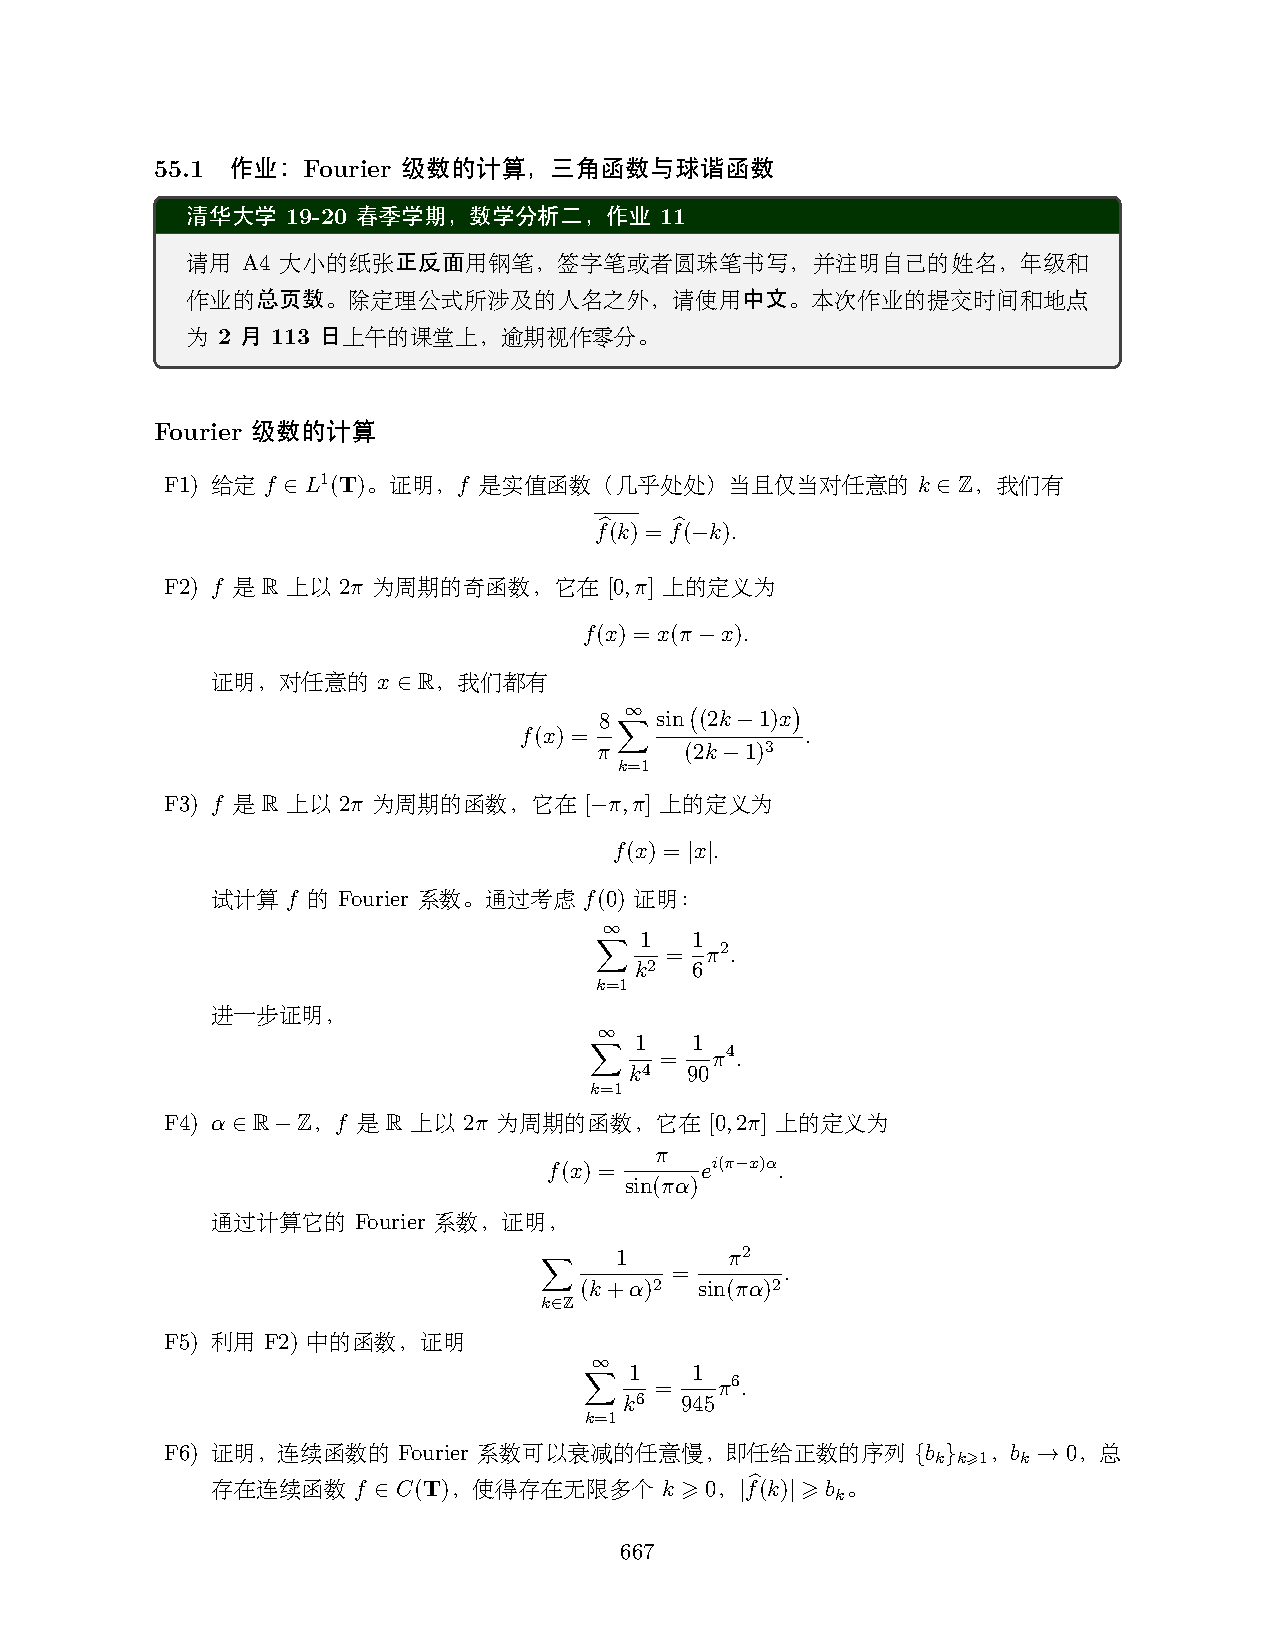
\includepdf[pages=-,pagecommand={\thispagestyle{empty}},scale=.94]{original.pdf}}

\begin{document}
\sourceintro{55.1 作业：Fourier性质、三角函数与球谐函数}{55.1}{667--673}
\section*{所用知识与记号}
第31讲链式法则、第46讲子流形测度、第52--55讲Hilbert基、Fourier唯一性与收敛；第20.1节的Stone--Weierstrass定理。球谐函数的分解、微分算子及归一化均在本篇证明，不借用表示论。Fourier约定$\widehat f(k)=(2\pi)^{-1}\int_{-\pi}^{\pi}f(x)e^{-ikx}\dd x$。圆周及球面的内积使用未归一化面积元。
\section{Fourier系数的性质}
\problem{F1}{给定$f\in L^1(\T)$，证明$f$几乎处处实值当且仅当$\widehat f(k)=\overline{\widehat f(-k)}$对所有$k$成立。}
直接共轭积分得$\widehat{\overline f}(k)=\overline{\widehat f(-k)}$，故正向成立。反向所有$f-\overline f$的Fourier系数为零，其Fejér平均均零，而Fejér平均在$L^1$中趋于函数自身，所以$f=\overline f$几乎处处。
\skipnote{F2--F5为指定函数的Fourier系数及$\zeta(2),\zeta(4),\zeta(6)$等具体级数求值，按纯计算题略去解答。四题的完整题干与公式见附录第667页。}
\problem{F6}{给定正数$b_k\to0$，证明存在连续$f$使无穷多个$k\ge0$满足$|\widehat f(k)|\ge b_k$。}
递归选择严格递增的正整数$k_j$，使$b_{k_j}\le2^{-j}$。令$f(x)=\sum_{j\ge1}2^{-j}e^{ik_jx}$，一致绝对收敛保证连续。可逐项积分，$\widehat f(k_j)=2^{-j}\ge b_{k_j}$。
\section{圆周上的三角函数}
令$\mathcal P_d^{(\ell)}$为$d$元复齐次$\ell$次多项式空间，$\mathcal H_d^{(\ell)}=\ker\Delta\cap\mathcal P_d^{(\ell)}$。零次齐次多项式包含常数。
\problem{s1}{证明单位圆周在参数$\theta$下面积元为$\dd\theta$，其$L^2$内积为$\int_0^{2\pi}f_1\overline{f_2}\dd\theta$。}
参数$(\cos\theta,\sin\theta)$的速度长为$1$，弧长元即$\dd\theta$。原文集合的环境$\R^3$应为$\R^2$。
\problem{s2}{证明二维极坐标中$\Delta=\partial_r^2+r^{-1}\partial_r+r^{-2}\partial_\theta^2$。}
链式法则给出$\partial_x=\cos\theta\partial_r-r^{-1}\sin\theta\partial_\theta$、$\partial_y=\sin\theta\partial_r+r^{-1}\cos\theta\partial_\theta$。平方相加时二阶交叉项抵消；系数被求导的项合成$r^{-1}\partial_r$，二阶角项为$r^{-2}\partial_\theta^2$。
\problem{s3}{证明$\Delta_\T=\partial_\theta^2$在光滑周期函数上的内积对称性。}
两次分部积分，周期端点值及一阶导数使边界项抵消，得$\int f_1''\overline{f_2}=\int f_1\overline{f_2''}$。这里只证明题目所述的对称性；无界算子的自伴性还涉及定义域。
\problem{s4}{令$(g\bullet f)(x)=f(g^{-1}x)$，$g\in SO(2)$，证明该作用保持$L^2$内积。}
旋转对应$\theta\mapsto\theta-\alpha$，周期积分平移不变，结论成立。
\problem{s5}{证明旋转保持二维调和函数。}
正交链式法则给出$\Delta(f\circ g^{-1})=(\Delta f)\circ g^{-1}$，因为两个$g^{-1}$矩阵系数的收缩为单位矩阵。
\problem{s6}{证明$\dim\mathcal P_2^{(\ell)}=\ell+1$，且旋转保持此空间。}
单项式$x^jy^{\ell-j}$、$0\le j\le\ell$为基。线性坐标代换保持次数与齐次性。原文求和指标$\ell_1+\ell_1$应为$\ell_1+\ell_2$。
\problem{s7}{证明$\Delta:\mathcal P_2^{(\ell)}\to\mathcal P_2^{(\ell-2)}$在$\ell\ge2$时满射。}
使用同样适用于三维的代数构造。写$\Delta=\partial_1^2+\Delta'$，令$I$对$x_1$作两次不带常数的积分，即$I(x_1^aQ)=x_1^{a+2}Q/[(a+1)(a+2)]$。$I$与$\Delta'$交换。给定齐次$Q$，取
\[P=I\sum_{j=0}^{J}(-I\Delta')^jQ,\]
其中$J$足够大使$(\Delta')^{J+1}Q=0$。则$\Delta P=(1+I\Delta')\sum_{j=0}^{J}(-I\Delta')^jQ=Q$。各项均为$\ell$次齐次，故满射。
\problem{s8}{证明$\ell\ge1$时$\dim\mathcal H_2^{(\ell)}=2$，且在旋转作用下不变。}
当$\ell\ge2$，秩零化度为$(\ell+1)-(\ell-1)=2$；$\ell=1$直接为所有线性式。旋转与$\Delta$交换，故保持核。$\ell=0$时维数为$1$，单独处理。
\problem{s9}{若$P$为$\ell$次齐次调和多项式，$p=P|_\T$，证明$-\Delta_\T p=\ell^2p$。}
$P(r,\theta)=r^\ell p(\theta)$，代入s2得到$\Delta P=r^{\ell-2}(\ell^2p+p'')$，从而结论成立。
\problem{s10}{证明$\ell\ge1$时$\mathcal H_2^{(\ell)}$由$(x+iy)^\ell,(x-iy)^\ell$生成。}
这两个多项式的$\partial_x^2+\partial_y^2$相消，且在圆周上限制为$e^{i\ell\theta},e^{-i\ell\theta}$，线性无关。结合s8维数即得。
\problem{s11}{令$e_k|_\T=e^{ik\theta}$，证明$\{e_k/\sqrt{2\pi}:k\in\Z\}$为$L^2(\T,\dd\theta)$的Hilbert基。}
积分给出正交且归一化；三角多项式在连续周期函数中由Fejér定理一致稠密，而连续函数在$L^2$稠密，所以该正交系完备。
\section{球面上的多项式分解}
令$S^2\subset\R^3$为单位球面，$\mathcal P^{(\ell)}=\mathcal P_3^{(\ell)}$，$\mathcal H^{(\ell)}=\mathcal H_3^{(\ell)}$。
\problem{S1}{证明球坐标下面积元为$\sin\vartheta\dd\vartheta\dd\phi$，并据此写出$L^2$内积。}
参数映射的两切向量正交，长度为$1,\sin\vartheta$，Gram行列式平方根为$\sin\vartheta$。故内积为$\int_0^\pi\int_0^{2\pi}f_1\overline{f_2}\sin\vartheta\dd\phi\dd\vartheta$。
\problem{S2}{证明
\[\Delta=\partial_r^2+2r^{-1}\partial_r+r^{-2}\Delta_{S^2},\qquad\Delta_{S^2}=\partial_\vartheta^2+\cot\vartheta\partial_\vartheta+\sin^{-2}\vartheta\partial_\phi^2.\]}
正交坐标的梯度为$e_r\partial_rf+e_\vartheta r^{-1}\partial_\vartheta f+e_\phi(r\sin\vartheta)^{-1}\partial_\phi f$。各坐标面积与体积之比（或直接链式法则）给出散度，得到
\[\Delta f=\frac1{r^2}\partial_r(r^2f_r)+\frac1{r^2\sin\vartheta}\partial_\vartheta(\sin\vartheta f_\vartheta)+\frac1{r^2\sin^2\vartheta}f_{\phi\phi}.\]
展开即得。
\problem{S3}{证明$\Delta_{S^2}$在光滑函数上的内积对称性。}
按S2分部积分得
\[(\Delta_{S^2}f,g)=-\int_{S^2}\left(f_\vartheta\overline{g_\vartheta}+\sin^{-2}\vartheta f_\phi\overline{g_\phi}\right)\dd\sigma=(f,\Delta_{S^2}g).\]
可先去掉极点小帽再取极限；光滑性使$\sin\vartheta f_\vartheta\overline g$的边界项趋零，$\phi$方向周期边界抵消。
\problem{S4}{证明$SO(3)$在球面上的拉回作用保持$L^2$内积。}
正交变换保持切向量Gram矩阵，从而保持球面面积元，换元即得。
\problem{S5}{证明$SO(3)$保持三维调和函数。}
与s5相同，正交链式法则给出$\Delta(f\circ g^{-1})=(\Delta f)\circ g^{-1}$。
\problem{S6}{证明$\dim\mathcal P^{(\ell)}=(\ell+1)(\ell+2)/2$，且该空间在旋转下不变。}
基由$x_1^ax_2^bx_3^c$、$a+b+c=\ell$给出，个数为$\binom{\ell+2}2$。线性坐标代换保持齐次次数。原文指标$\ell_1+\ell_1+\ell_3$应为$\ell_1+\ell_2+\ell_3$。
\problem{S7*}{证明$\Delta:\mathcal P^{(\ell)}\to\mathcal P^{(\ell-2)}$满射。}
使用s7的构造，这次$\Delta'=\partial_2^2+\partial_3^2$。它反复作用会使$x_2,x_3$总次数降到负数，故仍为有限和，得到同一右逆。
\problem{S8}{证明$\dim\mathcal H^{(\ell)}=2\ell+1$，且在旋转作用下不变。}
$\ell\ge2$时由满射和维数相减得到$\binom{\ell+2}2-\binom\ell2=2\ell+1$；$\ell=0,1$直接验证。旋转与$\Delta$交换，故核不变。
\problem{S9}{原文要求对$P\in\mathcal P^{(\ell)}$证明$\Delta(r^{2k}P)=2k(2\ell-2k+1)r^{2k-2}P+r^{2k}\Delta P$。}
\fix{系数有误，正确为$2k(2\ell+2k+1)$。例如$P=1,k=1$时左边$\Delta r^2=6$，原系数为$-2$。}
利用$\nabla r^{2k}=2kr^{2k-2}x$、$\Delta r^{2k}=2k(2k+1)r^{2k-2}$及Euler式$x\cdot\nabla P=\ell P$，乘积法则给出
\[\Delta(r^{2k}P)=r^{2k}\Delta P+[2k(2k+1)+4k\ell]r^{2k-2}P.\]
\problem{S10*}{证明若$P\in\mathcal P^{(\ell)}$且$r^2P$调和，则$P=0$。}
若$P\ne0$，写$P=r^{2j}Q$，其中$r^2$不整除$Q$。对$r^{2j+2}Q$用修正S9，去掉公因子$r^{2j}$得到$cQ+r^2\Delta Q=0$，$c=2(j+1)(2\deg Q+2j+3)>0$。这使$r^2$整除$Q$，矛盾。
\problem{S11}{证明$\mathcal P^{(\ell)}=\mathcal H^{(\ell)}\oplus r^2\mathcal P^{(\ell-2)}$，并迭代为各次调和空间的和。}
两者交为零由S10；维数之和$2\ell+1+\binom\ell2=\binom{\ell+2}2$，故直和等于全空间。对次数$\ell-2$的空间重复即可。
\problem{S12}{令$H_\ell=\mathcal H^{(\ell)}|_{S^2}$、$P_\ell=\mathcal P^{(\ell)}|_{S^2}$。证明$H_\ell$为有限维Hermite空间、内积旋转不变，且$P_\ell=H_\ell\oplus H_{\ell-2}\oplus\cdots$。}
齐次多项式由球面限制唯一决定，因为$P(r\omega)=r^\ell P(\omega)$，所以限制映射单射；正定性由非零连续函数的平方积分严格正。S4给出旋转不变。把S11限制到$r=1$得到分解；唯一性也可把各项乘适当$r^{2j}$恢复为同次齐次分解。之后S17与S3还说明各项相互正交。
\section{角动量算子}
\problem{S13}{限制与齐次扩张互逆，$\Ext(Y)=r^\ell Y$。令$X_1=x_3\partial_2-x_2\partial_3$、$X_2=x_1\partial_3-x_3\partial_1$、$X_3=x_2\partial_1-x_1\partial_2$，$D_i=\Res X_i\Ext$。证明其保持$P_\ell,H_\ell$，并求球坐标式。}
线性系数一阶微分保持齐次次数；$[X_i,\Delta]=0$，故保持调和性。将$X_i$投到$e_\vartheta,e_\phi$上得到
\[D_1=\sin\phi\partial_\vartheta+\cos\phi\cot\vartheta\partial_\phi,\quad D_2=-\cos\phi\partial_\vartheta+\sin\phi\cot\vartheta\partial_\phi,\quad D_3=-\partial_\phi.\]
例如$X_1=(0,x_3,-x_2)$与$e_\vartheta$内积为$r\sin\phi$，与$e_\phi$内积为$r\cos\vartheta\cos\phi$，除以相应坐标长度即得第一式，其余同理。
\problem{S14}{令$J_i=iD_i$、$J_\pm=J_1\pm iJ_2$。证明$J_i$对称、$J_+$与$J_-$互为形式伴随。}
$D_i$是保持球面面积的旋转流的导数。对不变内积求导得$(D_if,g)=-(f,D_ig)$；因内积第二项反线性，乘$i$后得到$(J_if,g)=(f,J_ig)$。再对$J_1\pm iJ_2$展开，伴随中的$i$共轭变号，即得结论。
\problem{S15}{令$J^2=\sum_iJ_i^2=J_+J_-+J_3^2-J_3$。证明$J^2=-\Delta_{S^2}$。}
由球坐标式直接得到
\[D_1^2+D_2^2=\partial_\vartheta^2+\cot\vartheta\partial_\vartheta+\cot^2\vartheta\partial_\phi^2,\qquad D_3^2=\partial_\phi^2.\]
因为$1+\cot^2=\csc^2$，乘$i^2=-1$即得。另由$[J_1,J_2]=iJ_3$展开$J_+J_-$得到所列Casimir等式。
\problem{S16}{对$Y\in P_\ell$及$P=r^\ell Y$，证明$\Delta P=0$等价于$\Delta_{S^2}Y=-\ell(\ell+1)Y$。}
S2给出$\Delta(r^\ell Y)=r^{\ell-2}[\ell(\ell+1)Y+\Delta_{S^2}Y]$，故等价。
\problem{S17}{证明$-\Delta_{S^2}|_{H_\ell}=\ell(\ell+1)\operatorname{Id}$。}
每个$Y\in H_\ell$来自调和齐次多项式，直接用S16。
\problem{S18*}{原文声称$\Span\{H_\ell:\ell=1,2,\ldots\}$在$L^2(S^2)$稠密。}
\fix{必须包含$\ell=0$。原空间中每个函数与常数正交，因为S3、S17给出$\ell(\ell+1)\int Y=0$，故不能逼近常数。原文随后把特征空间维数写成$\ell(\ell+1)$也有误，应为$2\ell+1$。}
修正后，球面上坐标多项式的限制构成含常数、分离点、对共轭封闭的代数，Stone--Weierstrass给出在$C(S^2)$中一致稠密。S11使任意多项式限制为有限个$H_\ell$之和。连续函数在有限测度紧球面上$L^2$稠密，因而得到修正版。
\section{显式球谐函数及相位勘误}
对$0\le m\le\ell$，原题定义
\[Q_{\ell,m}(u)=\frac{\dd^{\ell+m}}{\dd u^{\ell+m}}(1-u^2)^\ell,\quad Z_\ell^m(\vartheta)=\sin^m\vartheta\,Q_{\ell,m}(\cos\vartheta),\]
\[C_{m,\ell}=\frac{(-1)^{\ell+m}}{2^\ell\ell!}\sqrt{\frac{2\ell+1}{4\pi}}\sqrt{\frac{(\ell-m)!}{(\ell+m)!}},\qquad Y_\ell^m=C_{m,\ell}Z_\ell^m e^{im\phi}.\]
对$m<0$，原题令$Y_\ell^m=\overline{Y_\ell^{-m}}$。以下先保留此原始约定，记$\epsilon_m=1$（$m\ge0$）、$\epsilon_m=(-1)^m$（$m<0$），并令$\mathcal Y_\ell^m=\epsilon_mY_\ell^m$为修正相位后的球谐函数。
\problem{S19}{证明以上所有$Y_\ell^m$均为非零光滑球面函数。}
$Q_{\ell,m}$为非零$\ell-m$次多项式，且仅含与$\ell-m$同奇偶的次数。故$r^\ell Y_\ell^m$可写成非零常数乘
\[(x_1+ix_2)^m\sum_jc_jx_3^{\ell-m-2j}(x_1^2+x_2^2+x_3^2)^j.\]
这是齐次多项式，故球面限制光滑，极点的坐标奇异完全消失；非零性由多项式首项或$Q$非零得到。负$m$取共轭即可。
\problem{S20}{写出$\ell=0,1,2$的九个$Y_\ell^m$，并证明各自范数为$1$且相互正交。}
令$u=\cos\vartheta,v=\sin\vartheta$，按\emph{原题负指标相位}得到
\begin{align*}
Y_0^0&=1/\sqrt{4\pi},&Y_1^0&=\sqrt{3/(4\pi)}u,\\
Y_1^{\pm1}&=-\sqrt{3/(8\pi)}ve^{\pm i\phi},&Y_2^0&=\sqrt{5/(16\pi)}(3u^2-1),\\
Y_2^{\pm1}&=-\sqrt{15/(8\pi)}uve^{\pm i\phi},&Y_2^{\pm2}&=\sqrt{15/(32\pi)}v^2e^{\pm2i\phi}.
\end{align*}
不同$m$的正交性由$\phi$积分；同$m$不同$\ell$由$u$奇偶性或$\int_{-1}^1(3u^2-1)\dd u=0$。归一化逐式用$\int_{-1}^1u^{2j}\dd u=2/(2j+1)$，$j=0,1,2$，以及$\int_0^{2\pi}\dd\phi=2\pi$得到，例如$\norm{Y_2^2}^2=(15/16)\int_{-1}^1(1-u^2)^2\dd u=1$。
\problem{S21}{原题要求证明$-\Delta Y_\ell^m=\ell(\ell+1)Y_\ell^m$、$J_3Y_\ell^m=mY_\ell^m$、$J_\pm Y_\ell^m=\sqrt{(\ell\mp m)(\ell\pm m+1)}Y_\ell^{m\pm1}$。}
\fix{前两式正确；后两式与原题负指标的共轭定义不相容。例如$J_+Y_1^{-1}=-\sqrt2Y_1^0$，原式却给正号。若负指标改为$\mathcal Y_\ell^m=(-1)^m\overline{Y_\ell^{-m}}$，所有标准升降公式成立。原约定下应额外乘$\epsilon_m/\epsilon_{m\pm1}$。}
以下证明而非借用标准球谐理论。令$R=(1-u^2)^\ell$，恒等式$(1-u^2)R'=-2\ell uR$求导$\ell+m+1$次，得
\[(1-u^2)Q''-2(m+1)uQ'+(\ell-m)(\ell+m+1)Q=0.\]
置$Z=(1-u^2)^{m/2}Q$并用乘积法则整理得到
\[\frac\dd{\dd u}[(1-u^2)Z']+\left[\ell(\ell+1)-\frac{m^2}{1-u^2}\right]Z=0.\]
这是S2角算子作用于$Ze^{im\phi}$的方程，证明第一式；第二式直接对$\phi$求导。又
\[J_+=e^{i\phi}(\partial_\vartheta+i\cot\vartheta\partial_\phi),\quad J_-=e^{-i\phi}(-\partial_\vartheta+i\cot\vartheta\partial_\phi).\]
对$m\ge0$，有
\[\partial_\vartheta(\sin^m\vartheta Q)-m\cot\vartheta\sin^m\vartheta Q=-\sin^{m+1}\vartheta Q'.\]
再用$-C_{m,\ell}/C_{m+1,\ell}=\sqrt{(\ell-m)(\ell+m+1)}$，得升公式。降公式对$m\ge1$可用上面的$Q$微分方程：令$Q_-=R^{(\ell+m-1)}$，其方程给出
\[(1-u^2)Q'-2muQ=-(\ell+m)(\ell-m+1)Q_-;\]
与$C_{m,\ell}/C_{m-1,\ell}=-1/\sqrt{(\ell+m)(\ell-m+1)}$合并，得正系数降公式。$m=0$及负$m$使用$J_+\overline h=-\overline{J_-h}$处理，恰产生已说明的相位符号。两端超出$|m|\le\ell$的项系数为零。
\problem{S22}{证明$Y_\ell^m\in H_\ell$。}
S19已经给出其$\ell$次齐次多项式扩张；S21的角特征方程结合S16说明这个多项式调和。因此属于$H_\ell$，不必预先假设完整谱理论。
\problem{S23}{证明不同$(\ell,m)$的$Y_\ell^m$正交。}
若$\ell\ne\ell'$，$-\Delta_{S^2}$对称且特征值$\ell(\ell+1)$不同，所以内积为零；若$\ell=\ell'$但$m\ne m'$，用对称算子$J_3$的不同特征值，同理。相位改变不影响正交性。
\problem{S24*}{固定$\ell$，证明$\norm{Y_\ell^m}_2$与$m$无关。}
对修正相位的$\mathcal Y$，S14给出
\[\norm{J_+\mathcal Y^m}^2=(\mathcal Y^m,J_-J_+\mathcal Y^m)=(\ell-m)(\ell+m+1)\norm{\mathcal Y^m}^2.\]
升公式左端也等于同一正系数乘$\norm{\mathcal Y^{m+1}}^2$，故邻项范数相等；遍历$-\ell\le m<\ell$即可。原始$Y$与$\mathcal Y$只差模$1$相位，范数相同。
\problem{S25}{证明每个$Y_\ell^m$范数为$1$。}
只需算$m=\ell$。因$Q_{\ell,\ell}=(-1)^\ell(2\ell)!$，
\[|Y_\ell^\ell|^2=\frac{2\ell+1}{4\pi}\frac{(2\ell)!}{2^{2\ell}(\ell!)^2}\sin^{2\ell}\vartheta.\]
分部积分递推给出$\int_0^\pi\sin^{2\ell+1}\vartheta\dd\vartheta=2^{2\ell+1}(\ell!)^2/(2\ell+1)!$，再乘$2\pi$正好得$1$。S24传递给所有$m$。结合维数$2\ell+1$和S18修正版，全部这些函数构成$L^2(S^2)$的Hilbert基；使用原相位或修正相位均成立。
\originalpages
\end{document}
